\section{问题一模型的建立与求解}
\label{sec:problem1}

\subsection{问题分析与建模思路}

问题一包含数据质量评价与训练数据配比优化两个相互关联的任务。前者利用附件 A1--A3 的多维质量信号回答“文本本身具有怎样的质量结构”，后者利用附件 A4--A15 的配比实验回答“领域组成如何改变模型验证损失”。两类附件的统计对象和监督信息不同：质量附件以文本为观测单位，配比附件以训练配方为观测单位，二者不能逐行拼接。因此，本文分别建立质量评价模型和配比响应模型，再借助 A16、A18 将质量域映射到配方域，作为解释性联系而非额外监督标签。

设第 $i$ 个配方域的比例与领域质量分别为 $p_i$ 和 $q_i$。由于 $\sum_i p_iq_i$ 是 $p_i$ 的线性组合，若将其与全部 Scheff\'e 一次项同时放入响应模型，就无法从现有配比实验中区分“领域组成效应”和“静态质量效应”。此外，A18 只提供文本及领域标签，并不包含 A1--A3 的完整质量信号。基于这两点，领域质量只用于解释配方特征和检验质量排序与训练收益是否一致；配比模型仍完全由配比--Loss 实验训练。

本问的技术路线为：先将 22 项异构质量信号转换到 $[0,1]$ 且统一为“越高越好”，再按质量含义构成五个语义块，通过稳定 CRITIC 权重与冲突自适应 Huber 估计得到样本质量 $Q_i$；随后在领域内稳健聚合并评估跨体系映射可靠性。配比侧则在单纯形上拟合二阶 Scheff\'e--Ridge 多输出响应面，通过 1M、60M 和 1B 实测配方检验模型的排序能力，最后在训练支持域内搜索近优可行配比，并用多起点和 bootstrap 量化求解不确定性。

上述两条建模链及其证据边界汇总于图~\ref{fig:p1_f00}。质量链输出样本分数、领域质量及映射可信度，配比链输出响应面、边际效应与近优可行配比；二者只在“质量--收益一致性检验”处作关联解释，避免把静态质量重复计入配比回归。图中的虚线表示验证、敏感性或关联分析，不参与主模型的数据传递。

\begin{figure}[htbp]
\centering
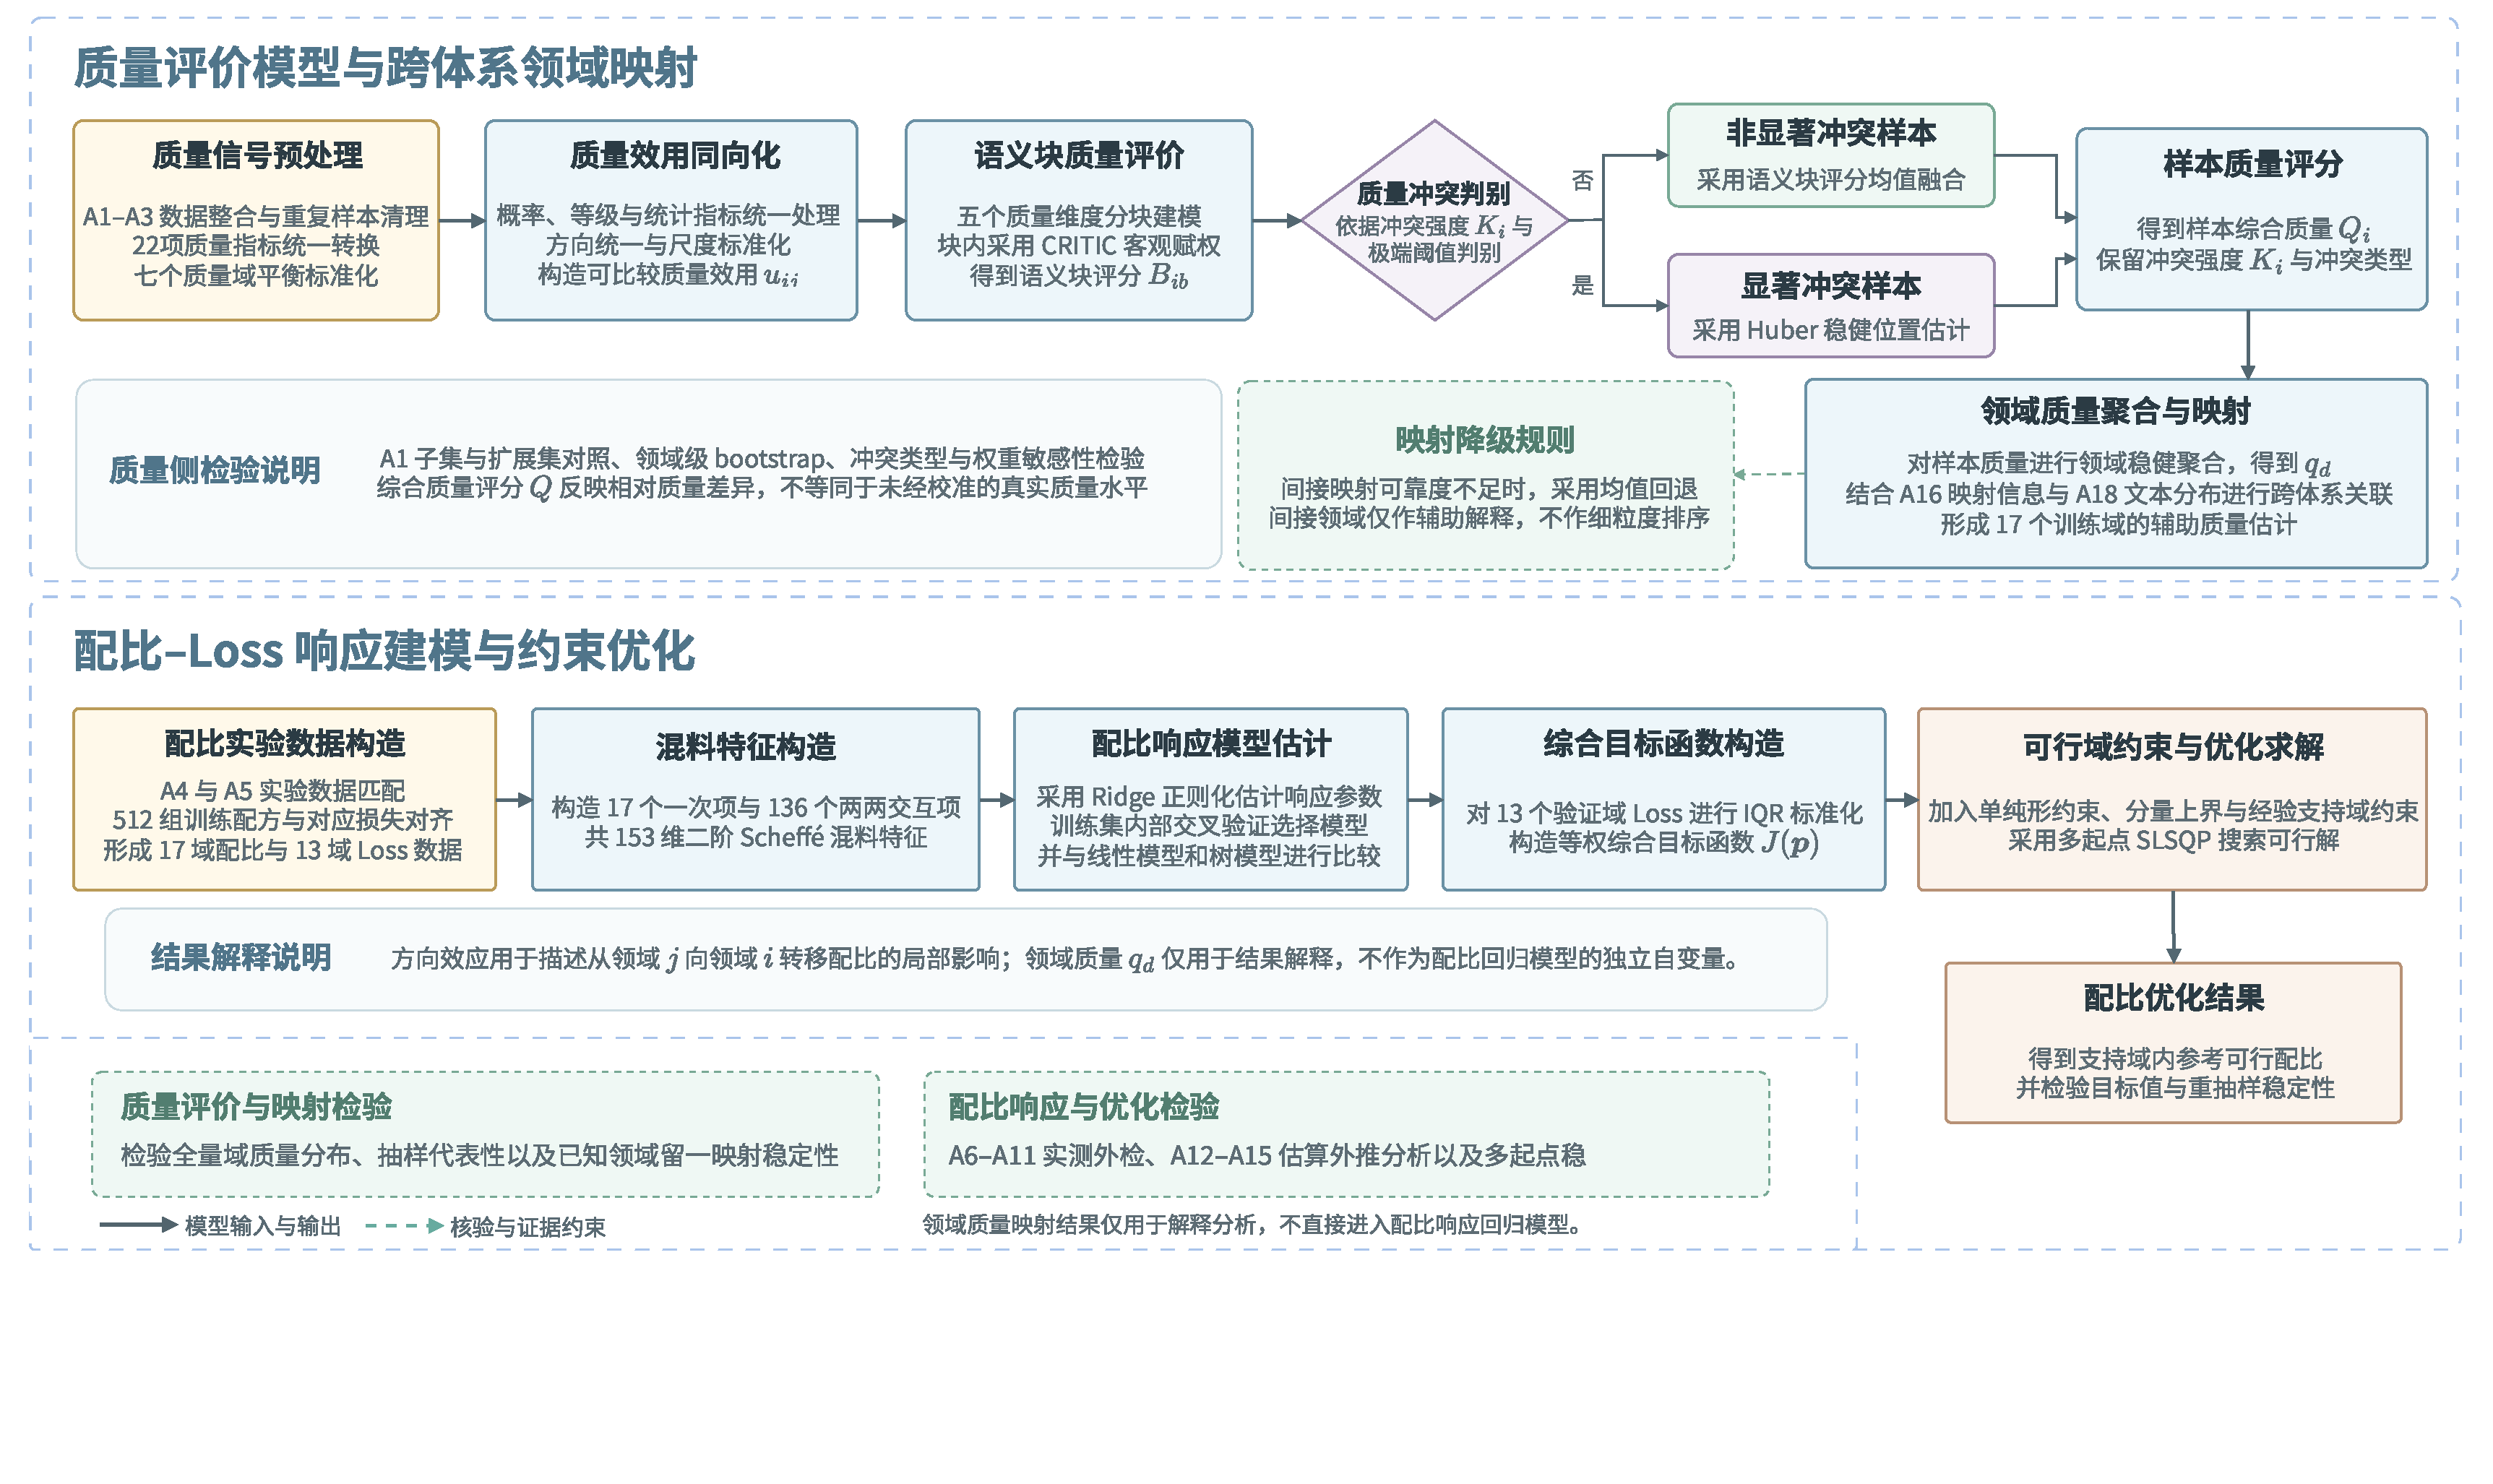
\includegraphics[width=0.97\linewidth]{images/no1/P1_F00R_问题一求解流程图.pdf}
\caption{问题一质量评价、领域映射与配比优化求解流程}
\label{fig:p1_f00}
\end{figure}

该框架最终形成四层可追溯结果：样本层保留 $Q_i$ 与冲突类型，领域层给出七域质量及 17 域映射区间，响应层保留 $\widehat L_k(\boldsymbol p)$ 与边际效应，决策层则给出带支持域和区间说明的近优配比族。后续各节依次给出这四层结果的构造与验证。

\subsection{输入、数据与证据边界}

\subsubsection{数据组织与预处理}

各附件的统计对象与分析角色见表~\ref{tab:p1_data_role}。质量侧以去重后的独立文本为统计单位；配比侧严格区分训练、实测检验和估算外推，测试数据不参与模型选择或正则化参数确定。

\begin{table}[htbp]
\centering
\small
\setlength{\tabcolsep}{5pt}
\caption{问题一主要数据及其分析角色}
\label{tab:p1_data_role}
\begin{tabular}{p{0.14\linewidth}p{0.29\linewidth}p{0.45\linewidth}}
\toprule
附件 & 统计对象 & 用途 \\
\midrule
A1--A3 & $51230$、$17523$、$203752$ 条质量记录 & 22 项质量信号转换、冲突分析、七域质量评价及扩展集检验 \\
A4/A5 & $512$ 组训练配方及 13 域 Loss & 配比响应面训练、内部交叉验证与模型选择 \\
A6/A7 & $256$ 组 1M 实测配方 & 同规模独立检验 \\
A8/A9 & $256$ 组 60M 实测配方 & 相同配方下的跨规模检验 \\
A10/A11 & $64$ 组 1B 实测配方 & 独立配方、独立规模检验 \\
A12--A15 & 10B、70B 各 $63$ 组估算配方 & 外推敏感性分析，不参与主模型训练与选模 \\
A16/A18 & 领域映射指引与 17 域文本样本 & 质量域到配方域的辅助映射及可靠性检验 \\
\bottomrule
\end{tabular}
\end{table}

A1 与 A2、A3 分别有 $1419$ 条 arXiv 记录和 $10000$ 条 GitHub 记录重合。本文以规范化领域名和样本标识联合去重，并核对重合记录的质量字段；未发现同标识质量冲突。最终质量参考集包含 $261086$ 条独立记录。原始数据中的少量非有限值保留为缺失，不做均值插补；样本评分仅使用其有效指标，并在块内重新归一权重，避免人为补值改变评价方向。

配比表与 Loss 表按 \texttt{index} 一一匹配。设第 $r$ 组实验中第 $i$ 个领域的原始份额为 $a_{ri}$，对存储精度引起的微小闭合误差作非负修正和重新归一化：
\begin{equation}
p_{ri}=\frac{\max(a_{ri},0)}{\sum_{j=1}^{17}\max(a_{rj},0)},
\qquad p_{ri}\ge 0,
\qquad \sum_{i=1}^{17}p_{ri}=1.
\label{eq:p1_closure}
\end{equation}
闭合后的最大行和误差为 $4.44\times10^{-16}$。训练配方包含 17 个领域比例和 13 个验证域 Loss；全部 17 个比例均作为组成变量保留，即使某些训练领域没有同名验证列，其作用仍可通过多输出响应面识别。

\subsection{模型建立}

\subsubsection{指标同向化与五语义块构建}

质量信号同时包含连续统计量、模型概率、有序分类输出和列表型评分。本文先将二分类 logits 转为正类概率，将六级分类 logits 转为有序期望，并将 QuRating 四个分量分别转换后取均值，最终得到题目要求的 22 项质量指标。所有效用均记为 $u_{ij}\in[0,1]$，且数值越大表示当前指标意义下的质量越高。

为避免 GitHub 等大样本领域主导经验标尺，对需作秩变换的指标 $j$，先在七个质量域内分别估计经验分布，再等权构造平衡参考分布
\begin{equation}
F_j^{\mathrm{bal}}(x)=\frac{1}{7}\sum_{d=1}^{7}F_{jd}(x).
\label{eq:p1_balanced_cdf}
\end{equation}
变换前按该平衡分布的 $0.5\%$ 和 $99.5\%$ 分位截尾。正向指标取 $u_{ij}=F_j^{\mathrm{bal}}(x_{ij})$，逆向指标取 $u_{ij}=1-F_j^{\mathrm{bal}}(x_{ij})$。词元熵与独特词比例具有边际收益递减特征，故采用饱和效用
\begin{equation}
u_{ij}=\min\left\{\frac{F_j^{\mathrm{bal}}(x_{ij})}{0.95},1\right\}.
\label{eq:p1_saturating_utility}
\end{equation}

文本长度、句子数和平均词长并非越大越好。对这类结构指标先作 $z_{ij}=\log(1+\max\{x_{ij},0\})$，再在高流畅、低广告且高整洁的可信样本中，以七域平衡方式估计中心 $m_j$ 和稳健尺度 $s_j$，定义中间型效用
\begin{equation}
u_{ij}=\exp\left[-\frac{(z_{ij}-m_j)^2}{2s_j^2}\right].
\label{eq:p1_mid_utility}
\end{equation}
数字字符比例具有明显领域依赖性：GitHub 中的数字和符号常属于正常代码结构，故使用中间型效用；其余自然语言领域仍按逆向指标处理。已经位于 $[0,1]$ 且方向明确的模型概率和有序期望不再重复作秩变换，以保留概率间距。

根据指标含义，22 项信号被划分为教育与领域价值、表达与整洁、推理与信息、噪声与重复、结构充分性五个语义块。先在块内融合，再在块间等权，可避免某一语义块仅因包含指标较多而获得更大总权重。

\subsubsection{稳定 CRITIC 赋权与质量冲突消解}

在同向化之后，指标间仍存在显著的信息重叠。本文在每个语义块内采用 CRITIC 思想确定客观权重\cite{diakoulaki1995critic}。为平衡领域样本量，每域最多等概率抽取 $10000$ 条记录。设指标 $j$ 的标准差为 $\sigma_j$，与同块指标 $h$ 的 Spearman 相关为 $r_{jh}$，则其信息量为
\begin{equation}
C_j=\sigma_j\sum_{h\in\mathcal J_b}(1-|r_{jh}|).
\label{eq:p1_critic_information}
\end{equation}
绝对相关同时惩罚强正相关和强负相关造成的信息重复。进一步在 500 次分层 bootstrap 中计算指标跨领域位置统计量的变异系数 $\mathrm{CV}_j$，得到稳定性修正后的块内权重
\begin{equation}
\omega_j=
\frac{C_j/(1+\mathrm{CV}_j)}
{\sum_{h\in\mathcal J_b}C_h/(1+\mathrm{CV}_h)},
\qquad \sum_{j\in\mathcal J_b}\omega_j=1.
\label{eq:p1_critic_weight}
\end{equation}

图~\ref{fig:p1_f01}给出 22 项同向化指标的相关结构及最终综合权重。图中若干指标形成明显相关簇，例如图书、百科和数学相似度之间高度相关；稳定 CRITIC 权重因此不会把同一类信息重复计入。平均词长的综合权重约为 $0.0899$，但五类语义块仍各占总评分的 $1/5$，不存在由单一指标直接决定综合质量的情形。

\begin{figure}[htbp]
\centering
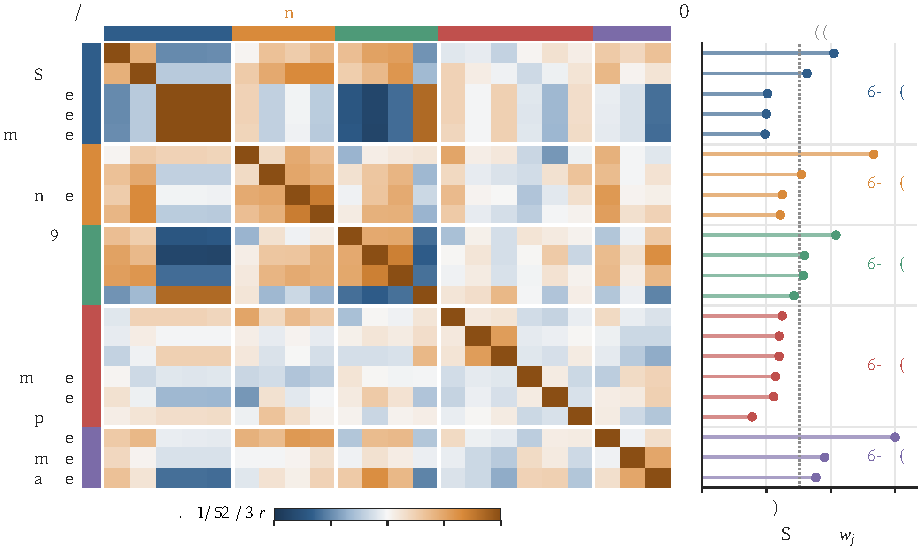
\includegraphics[width=0.98\linewidth]{images/no1/P1_F01_质量指标结构与权重.pdf}
\caption{质量指标相关结构与稳定 CRITIC 权重}
\label{fig:p1_f01}
\end{figure}

记 $\mathcal O_i$ 为样本 $i$ 的有效指标集合，$\mathcal J_b$ 为语义块 $b$ 的指标集合，则块评分为
\begin{equation}
B_{ib}=\frac{\sum_{j\in\mathcal J_b\cap\mathcal O_i}\omega_j u_{ij}}
{\sum_{j\in\mathcal J_b\cap\mathcal O_i}\omega_j}.
\label{eq:p1_block_score}
\end{equation}
若某块没有有效指标则记为缺失，不生成替代值。最终数据中没有样本出现整块缺失。

为识别“某一维度很高、另一维度很低”的内部矛盾，定义块间极差 $K_i=\max_b B_{ib}-\min_b B_{ib}$。当 $K_i$ 高于所属领域的 $90\%$ 分位，且同时满足 $\max_b B_{ib}\ge0.75$、$\min_b B_{ib}\le0.25$ 时，将样本标记为显著冲突。非冲突样本取有效块均值；冲突样本采用 Huber 稳健位置估计\cite{huber1964robust}：
\begin{equation}
Q_i=
\begin{cases}
|\mathcal B_i|^{-1}\displaystyle\sum_{b\in\mathcal B_i}B_{ib}, & i\notin\mathcal C,\\[6pt]
\displaystyle\arg\min_{q\in[0,1]}
\sum_{b\in\mathcal B_i}\frac{1}{|\mathcal B_i|}
\rho_{1.345}\!\left(\frac{B_{ib}-q}{s_{db}}\right), & i\in\mathcal C,
\end{cases}
\label{eq:p1_quality_score}
\end{equation}
其中 $\mathcal B_i$ 为有效块集合，$\mathcal C$ 为显著冲突样本集合，$s_{db}$ 为领域 $d$ 中块 $b$ 的 MAD 稳健尺度，$\rho_c$ 为 Huber 损失。该机制不删除冲突信息，而是同时保存 $K_i$、冲突方向和冲突标记，用于解释评分差异。

在 $261086$ 条记录中，显著冲突率为 $3.17\%$。图~\ref{fig:p1_f04}显示，较常见的冲突包括“推理信息高、结构充分低”“噪声重复高、结构充分低”和“表达整洁高、结构充分低”。Huber 修正对 $252816$ 个非冲突样本近似为零；对 $8270$ 个冲突样本，修正量均值约为 $0.0773$、中位数约为 $0.0376$，说明稳健估计主要调整内部不一致样本，而非改变全部样本的评分基线。

\begin{figure}[htbp]
\centering
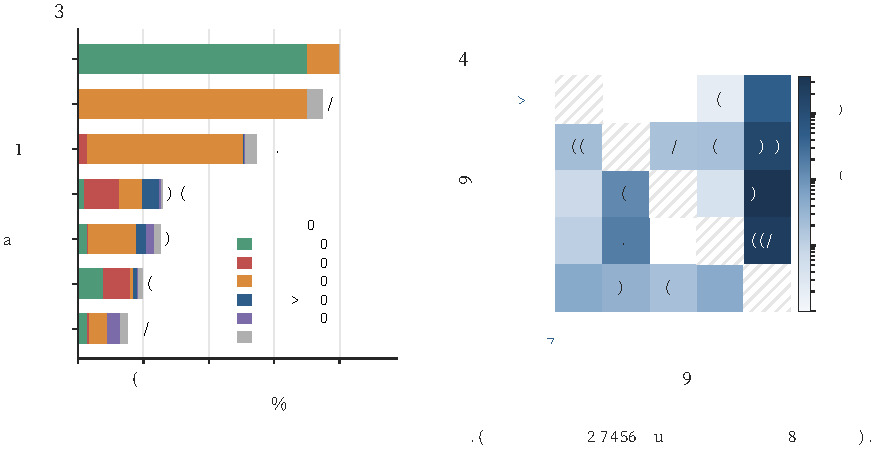
\includegraphics[width=0.96\linewidth]{images/no1/P1_F04_质量冲突机制与稳健消解.pdf}
\caption{质量冲突结构与 Huber 稳健修正效应}
\label{fig:p1_f04}
\end{figure}

\subsubsection{领域质量评价与跨体系映射}

样本质量范围为 $0.140735$--$0.880183$。对领域 $d$ 的样本集合 $\mathcal S_d$，本文使用领域内质量分数的 Huber 稳健均值，而不是简单均值或中位数：
\begin{equation}
q_d=\arg\min_q\sum_{i\in\mathcal S_d}
\rho_{1.345}\!\left(\frac{Q_i-q}{s_d}\right),
\label{eq:p1_domain_quality}
\end{equation}
其中 $s_d$ 为领域内 $Q_i$ 的 MAD 尺度。每个领域独立进行 500 次 bootstrap，取 $2.5\%$ 和 $97.5\%$ 分位作为不确定区间。表~\ref{tab:p1_quality}显示，C4 和 Common Crawl 在当前指标体系中的中心质量较高，GitHub 相对较低；这些结果反映质量信号空间中的相对位置，不等同于人工标注意义下的绝对文本价值。

\begin{table}[htbp]
\centering
\small
\setlength{\tabcolsep}{4pt}
\caption{七个质量域的稳健质量及显著冲突率}
\label{tab:p1_quality}
\begin{tabular}{lrrrr}
\toprule
领域 & 样本数 & 领域质量 $q_d$ & bootstrap 95\% 区间 & 冲突率/\% \\
\midrule
C4 & 10000 & 0.6192 & [0.6173, 0.6210] & 6.83 \\
Common Crawl & 9640 & 0.6083 & [0.6067, 0.6097] & 1.88 \\
arXiv & 17523 & 0.5688 & [0.5679, 0.5697] & 10.00 \\
Stack Exchange & 10000 & 0.5608 & [0.5591, 0.5624] & 3.14 \\
Book & 171 & 0.5100 & [0.4995, 0.5215] & 9.36 \\
Wikipedia & 10000 & 0.5067 & [0.5047, 0.5084] & 3.22 \\
GitHub & 203752 & 0.4304 & [0.4301, 0.4306] & 2.45 \\
\bottomrule
\end{tabular}
\end{table}

在使用扩展集给出最终域质量之前，需要检查 A1 抽样记录能否代表 A2/A3 的去重余集。图~\ref{fig:p1_f03}比较了 arXiv 和 GitHub 两域的经验分布差与分位数位移。两域的 KS 距离分别为 $0.025$ 和 $0.011$，Wasserstein 距离分别为 $0.0029$ 和 $0.0011$；Huber 均值差的 bootstrap 区间均跨越零。主体分布未见稳定偏移，但 arXiv 约第 $90$ 百分位处仍存在约 $0.076$ 的局部位移且区间较宽。因此，A1 对两域主体分布具有一定代表性，但不能据此宣称高质量尾部完全等价。

\begin{figure}[htbp]
\centering
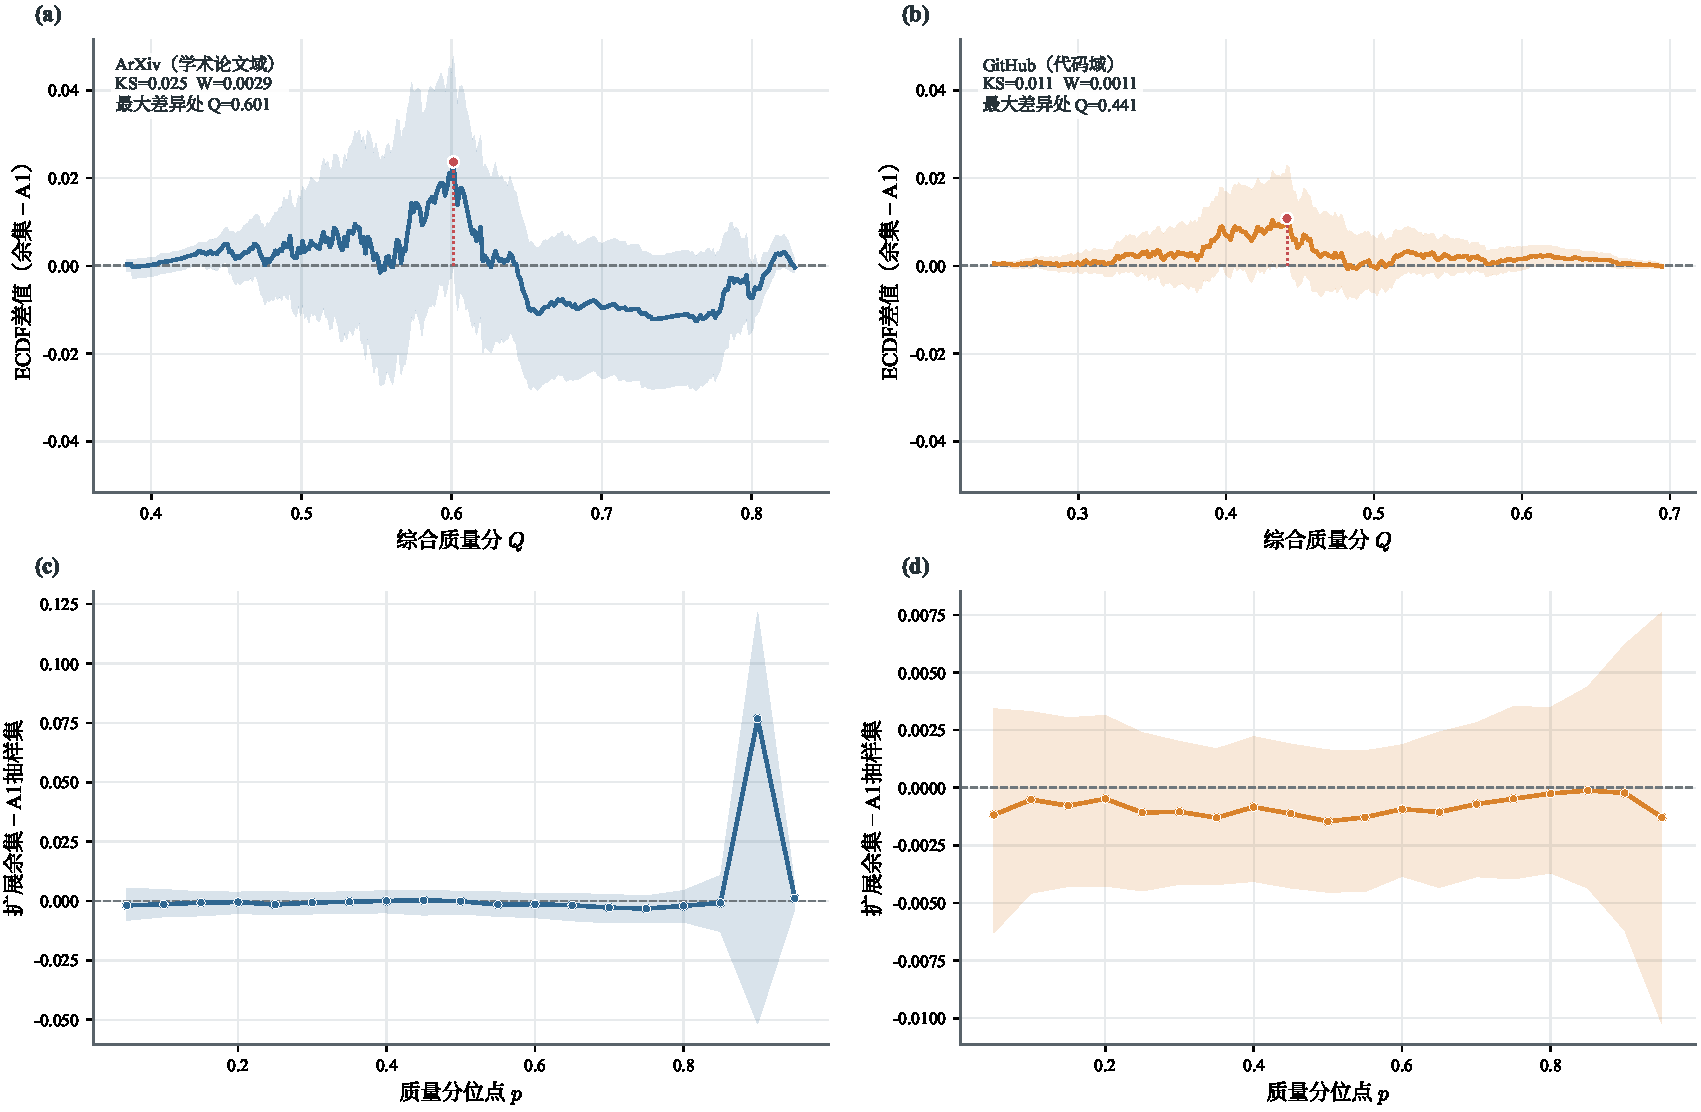
\includegraphics[width=0.98\linewidth]{images/no1/P1_F03_扩展集代表性诊断.pdf}
\caption{A1 抽样集相对扩展余集的分布代表性诊断}
\label{fig:p1_f03}
\end{figure}

质量附件覆盖七个领域，而配比模型使用 17 个 The Pile 领域。对 direct 和 near\_direct 映射，直接采用对应质量锚点；其余领域由 A18 文本的长度、字符、结构和重复特征与七个锚点进行距离匹配。设 $d_{md}$ 为配方域 $m$ 到质量域 $d$ 的标准化文本分布距离，温度参数为 $\tau$，则软映射权重与收缩估计为
\begin{equation}
w_{md}=\frac{\exp[-(d_{md}-d_{m,\min})/\tau]}
{\sum_{h=1}^{7}\exp[-(d_{mh}-d_{m,\min})/\tau]},
\quad
q_m=\lambda_m\sum_{d=1}^{7}w_{md}q_d+(1-\lambda_m)\bar q.
\label{eq:p1_mapping}
\end{equation}
其中 $\bar q$ 为七域质量均值。$\tau$ 只通过已知域留一误差选择；若留一排序达到预设可靠门槛，$\lambda_m$ 随 A18 样本量增加而增大、随最近锚点距离增加而减小，否则置为零。

最终选择 $\tau=5$，已知域留一 MAE 为 $0.056933$，但 Spearman 系数为 $-1$，不足以支持对推断域作稳定排序。因此，11 个推断域的 $\lambda_m$ 均置为零，并回退到公共参考质量 $\bar q=0.543464$。该值的 bootstrap 主区间约为 $[0.541887,0.545099]$；映射假设变化得到的 $[0.409869,0.677059]$ 仅作为敏感性包络，不能解释为真实质量的 95\% 置信区间。

图~\ref{fig:p1_f02}同时展示七域质量分布和 17 域映射证据。左侧山脊下方的点带为每域最多 500 个样本的固定随机抽样，用于辨认局部聚集、偏态和尾部结构；山脊上的三条标记依次对应 P5、中位数和 P95，因此点带仅辅助阅读，不参与领域质量估计。右侧连线宽度表示映射权重，颜色区分映射证据等级。17 个配方域中有 3 个直接映射、3 个近直接映射和 11 个推断映射。直接与近直接领域保留锚点差异；推断领域的共同数值只表示当前证据不足以区分，而非其真实质量相同。

\begin{figure}[htbp]
\centering
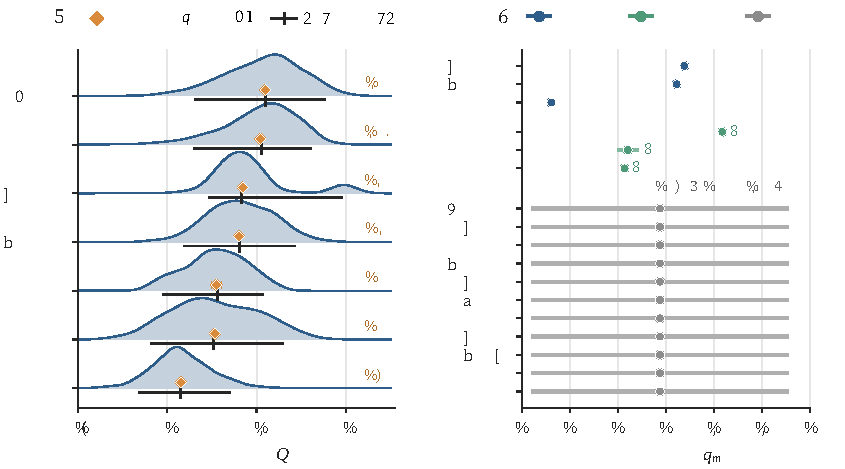
\includegraphics[width=0.98\linewidth]{images/no1/P1_F02_领域质量景观与映射.pdf}
\caption{七域质量分布、样本点带及其向 17 个配方域的映射}
\label{fig:p1_f02}
\end{figure}

为检验质量评分对聚合规则的敏感性，本文在不重新调参的条件下比较指标等权、块内等权、取消 Huber 和块中位数等方案。七域排序相对于主模型的最小 Kendall 系数为 $0.8095$，但样本高、低质量极端组的最低重合率仅为 $0.613$。因此，领域层面的总体差异具有一定稳定性，单个文本的精细排名则对融合规则更敏感，本文不将样本级排名解释为绝对质量顺序。

\subsubsection{Scheff\'e--Ridge 配比响应模型}

17 个领域份额满足式~\eqref{eq:p1_closure}，属于单纯形上的组成数据。普通含截距回归会因 $\sum_i p_i=1$ 产生线性依赖，故本文采用无截距二阶 Scheff\'e 混料模型\cite{scheffe1958mixtures}。对第 $k$ 个验证域，预测损失为
\begin{equation}
\widehat L_k(\boldsymbol p)
=\sum_{i=1}^{17}\beta_{ik}p_i
+\sum_{1\le i<j\le17}\beta_{ijk}p_ip_j,
\qquad k=1,\ldots,13.
\label{eq:p1_scheffe}
\end{equation}
模型包含 17 个一次项和 $\binom{17}{2}=136$ 个交互项，共 153 个特征。一次系数描述给定混料曲面中的基础响应，交互系数描述两个领域共同变化时的非加性关系；二者均是统计关联，不代表因果贡献。

记 $\boldsymbol X_s$ 为按训练折均方根尺度标准化后的 Scheff\'e 设计矩阵，$\boldsymbol Y\in\mathbb R^{n\times13}$ 为 13 个验证域 Loss。采用多输出 Ridge 稳定高维系数估计\cite{hoerl1970ridge}：
\begin{equation}
\widehat{\boldsymbol B}
=\arg\min_{\boldsymbol B}
\left\|\boldsymbol Y-\boldsymbol X_s\boldsymbol B\right\|_F^2
+\lambda\left\|\boldsymbol B\right\|_F^2.
\label{eq:p1_ridge}
\end{equation}
\subsection{模型求解}

\subsubsection{响应面选择与局部效应求解}

在 A4/A5 内按配比结构进行五折分层交叉验证，标准化仅在各训练折估计。正则化强度以 13 域 IQR 标准化均方根误差最小为准。二阶 Ridge 的内部 NRMSE 为 $0.3959$，略优于 Elastic Net 的 $0.3986$、线性 Ridge 的 $0.4108$、Extra Trees 的 $0.4307$ 和随机森林的 $0.4423$，故将二阶 Ridge 冻结为主响应面。树模型的秩相关较高，仍作为非线性对照，不据此宣称 Ridge 在所有指标上占优。

图~\ref{fig:p1_f09}(a)进一步并列给出误差与排序指标。图中 Pareto 列只按“NRMSE 越小、Spearman 越大”两个目标判定，Kendall 仅作为补充指标，因而二阶 Ridge 与 Extra Trees 同时位于前沿并不矛盾：Extra Trees 的 Spearman 为 $0.8545$，但 NRMSE 为 $0.4307$；二阶 Ridge 的 Spearman 为 $0.8285$，却将 NRMSE 降至 $0.3959$，同时保留连续可微、可解释且便于约束寻优的响应面。图~\ref{fig:p1_f09}(b)显示二阶 Ridge 在 $\alpha^*=0.0562$ 处取得最小误差，且其附近存在 NRMSE 距最优值不超过 $1\%$ 的稳定区间，说明选定正则强度并非由单个尖锐网格点偶然决定。

\begin{figure}[htbp]
\centering
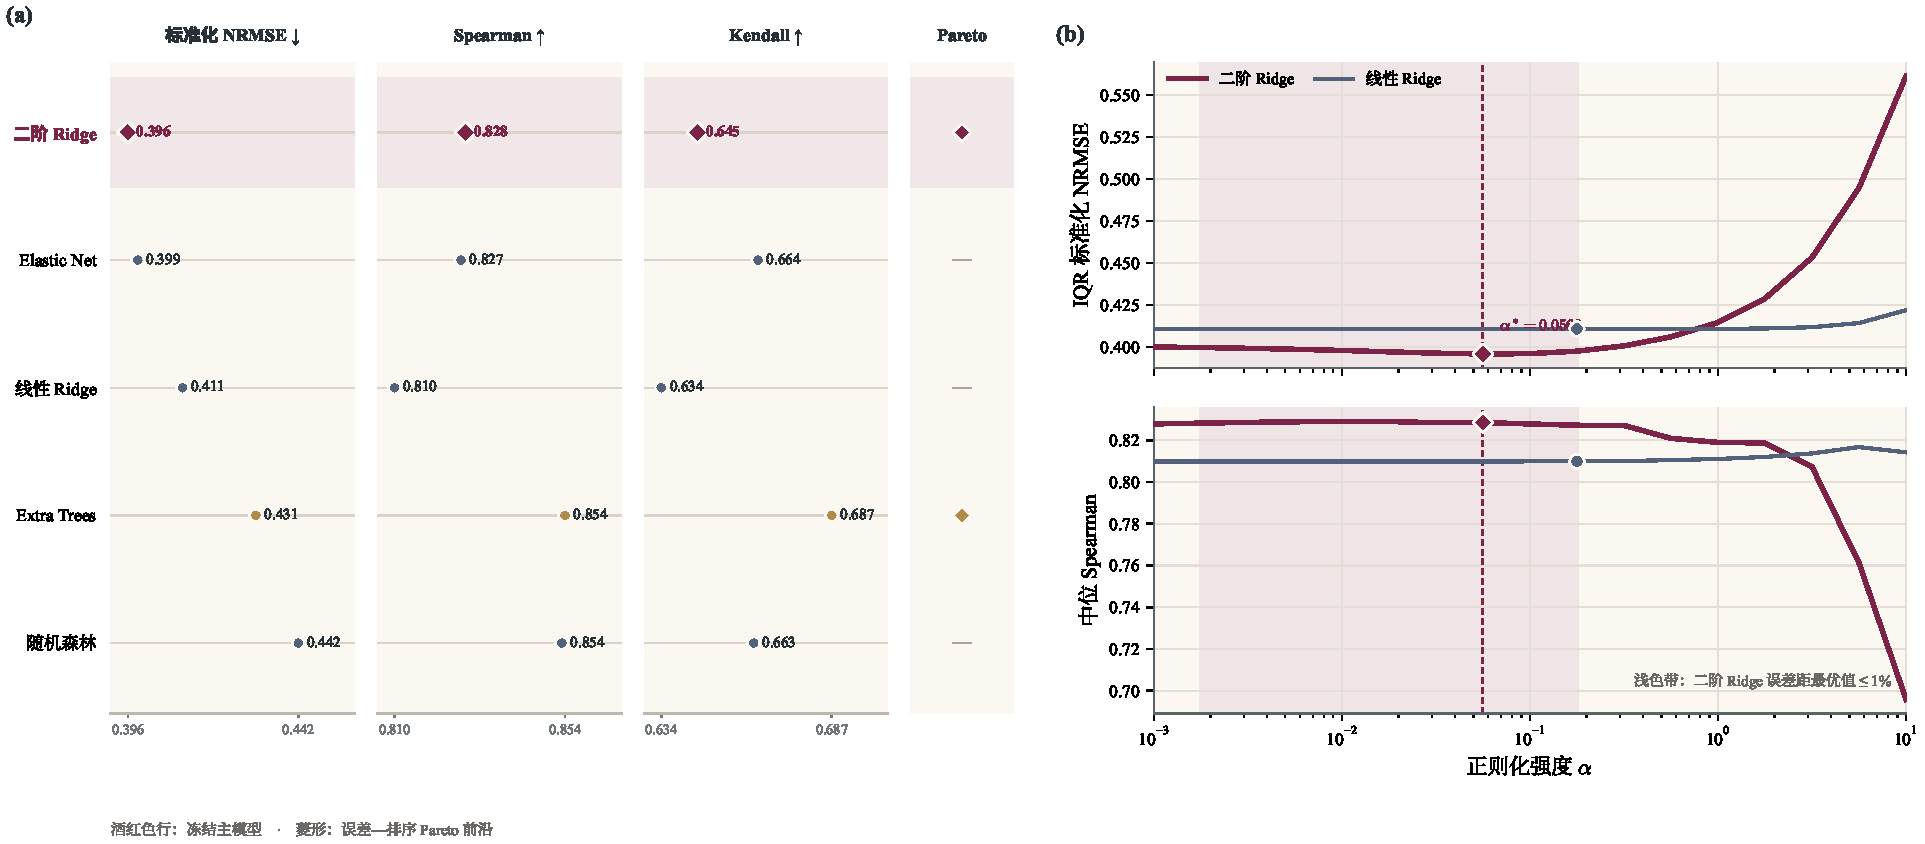
\includegraphics[width=0.98\linewidth]{images/no1/P1_F09_响应面选择与正则化诊断.pdf}
\caption{配比响应面的交叉验证选型与 Ridge 正则化诊断}
\label{fig:p1_f09}
\end{figure}

在组成约束下，单独增加某一份额必然压缩其他份额。为给出可解释的局部效应，在训练平均配比 $\boldsymbol p_{\mathrm{ref}}$ 处，将第 $i$ 个梯度相对于 17 域平均梯度中心化，并对 13 个验证域取均值。定义 Loss 下降方向的边际收益为
\begin{equation}
E_i=-\frac{1}{13}\sum_{k=1}^{13}
\left[
\frac{\partial\widehat L_k}{\partial p_i}
-\frac{1}{17}\sum_{j=1}^{17}
\frac{\partial\widehat L_k}{\partial p_j}
\right]_{\boldsymbol p=\boldsymbol p_{\mathrm{ref}}}.
\label{eq:p1_directional_effect}
\end{equation}
$E_i>0$ 表示在局部保持总比例不变时，向该领域转移份额与 Loss 下降相关。交互系数通过 500 次训练行 bootstrap 给出区间和符号稳定概率。

由于式~\eqref{eq:p1_directional_effect}只描述平均训练配比附近的一阶方向，本文进一步在 512 个训练配方上实施局部替换：按比例缩减其余 16 域，并向目标领域转入 $2\%$ 份额，再计算 13 个验证域的平均 Loss 降低量。图~\ref{fig:p1_f08}表明，同一领域的收益随参照配方显著变化。技术对话和数学推理的中位降低量分别为 $0.1072$ 和 $0.0657$，有利占比分别为 $91.2\%$ 和 $91.0\%$；商务邮件虽具有 $0.0973$ 的中位收益，但分布更宽，有利占比降至 $72.7\%$。哲学论文的中位效应仅为 $0.0044$，有利占比为 $52.3\%$，其 bootstrap 区间跨越零，不能据此给出稳定增配建议。

\begin{figure}[htbp]
\centering
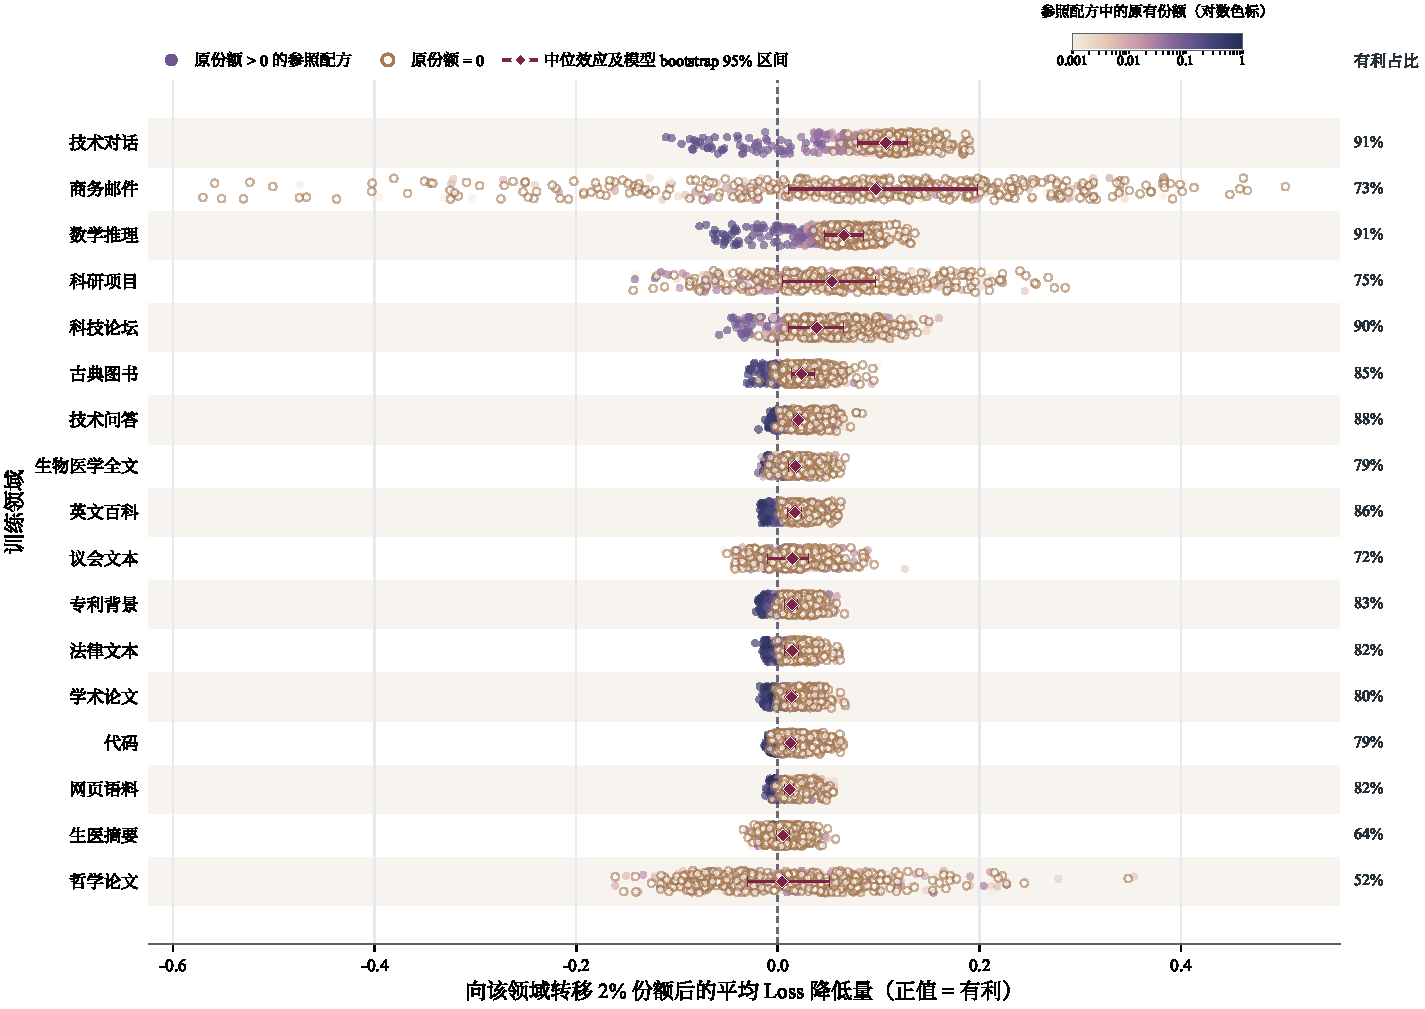
\includegraphics[width=0.94\linewidth]{images/no1/P1_F08_领域局部替换效应.pdf}
\caption{512 个训练配方上的领域局部替换效应}
\label{fig:p1_f08}
\end{figure}

图中多数领域的“原有份额--局部收益”相关为负，例如技术对话的 Spearman 系数为 $-0.662$，提示增配收益具有明显的起点依赖和边际递减特征。因此，领域效应应解释为给定组成附近的条件效应，而不能转化为脱离当前配方的固定领域排名。

\subsection{结果分析与模型验证}

\subsubsection{独立检验与跨尺度推广}

模型选择结束后，冻结的二阶 Ridge 一次性作用于 A6--A15。表~\ref{tab:p1_prediction}中的指标均为 13 个验证域的中位数；其中 1M、60M 和 1B 为实测检验，10B 和 70B 为附件中的估算标签。

\begin{table}[htbp]
\centering
\small
\setlength{\tabcolsep}{5pt}
\caption{配比响应面在不同规模数据上的检验结果}
\label{tab:p1_prediction}
\begin{tabular}{lrrrr}
\toprule
数据划分 & Spearman & Kendall & $R^2$ & 归一化后悔值 \\
\midrule
1M 实测 & 0.8582 & 0.6662 & 0.6366 & 0.1885 \\
60M 实测 & 0.8698 & 0.6829 & 0.6751 & 0.1404 \\
1B 实测 & 0.8503 & 0.6875 & 0.3236 & 0.0610 \\
10B 估算 & 0.5400 & 0.3811 & -231.3589 & 0.7426 \\
70B 估算 & 0.3937 & 0.2581 & -373.4716 & 0.8057 \\
\bottomrule
\end{tabular}
\end{table}

三个实测检验集的 Spearman 系数均处于 $0.850$--$0.870$，说明小模型配比响应能够较好保持候选方案的相对排序。1B 的 $R^2$ 降至 $0.3236$，表明绝对损失校准弱于排序能力。60M 和 1B 的 $R^2$ 使用各划分内部交叉拟合的仿射校准，而秩相关和归一化后悔值基于未校准预测，因此不同指标不能被理解为同一校准条件下的直接比较。

图~\ref{fig:p1_f05}给出三个实测尺度的折外预测。1M 和 60M 的预测主体接近理想线，1B 仍能保持总体顺序，但存在更明显的绝对偏差和少量大残差样本。因此，该响应面适合在实测尺度内筛选候选配比，而不宜将 1B 单点 Loss 解释为高精度绝对预测。10B、70B 的估算标签表现显著变差，只能说明远尺度外推存在风险，不能反向用于调参。

\begin{figure}[htbp]
\centering
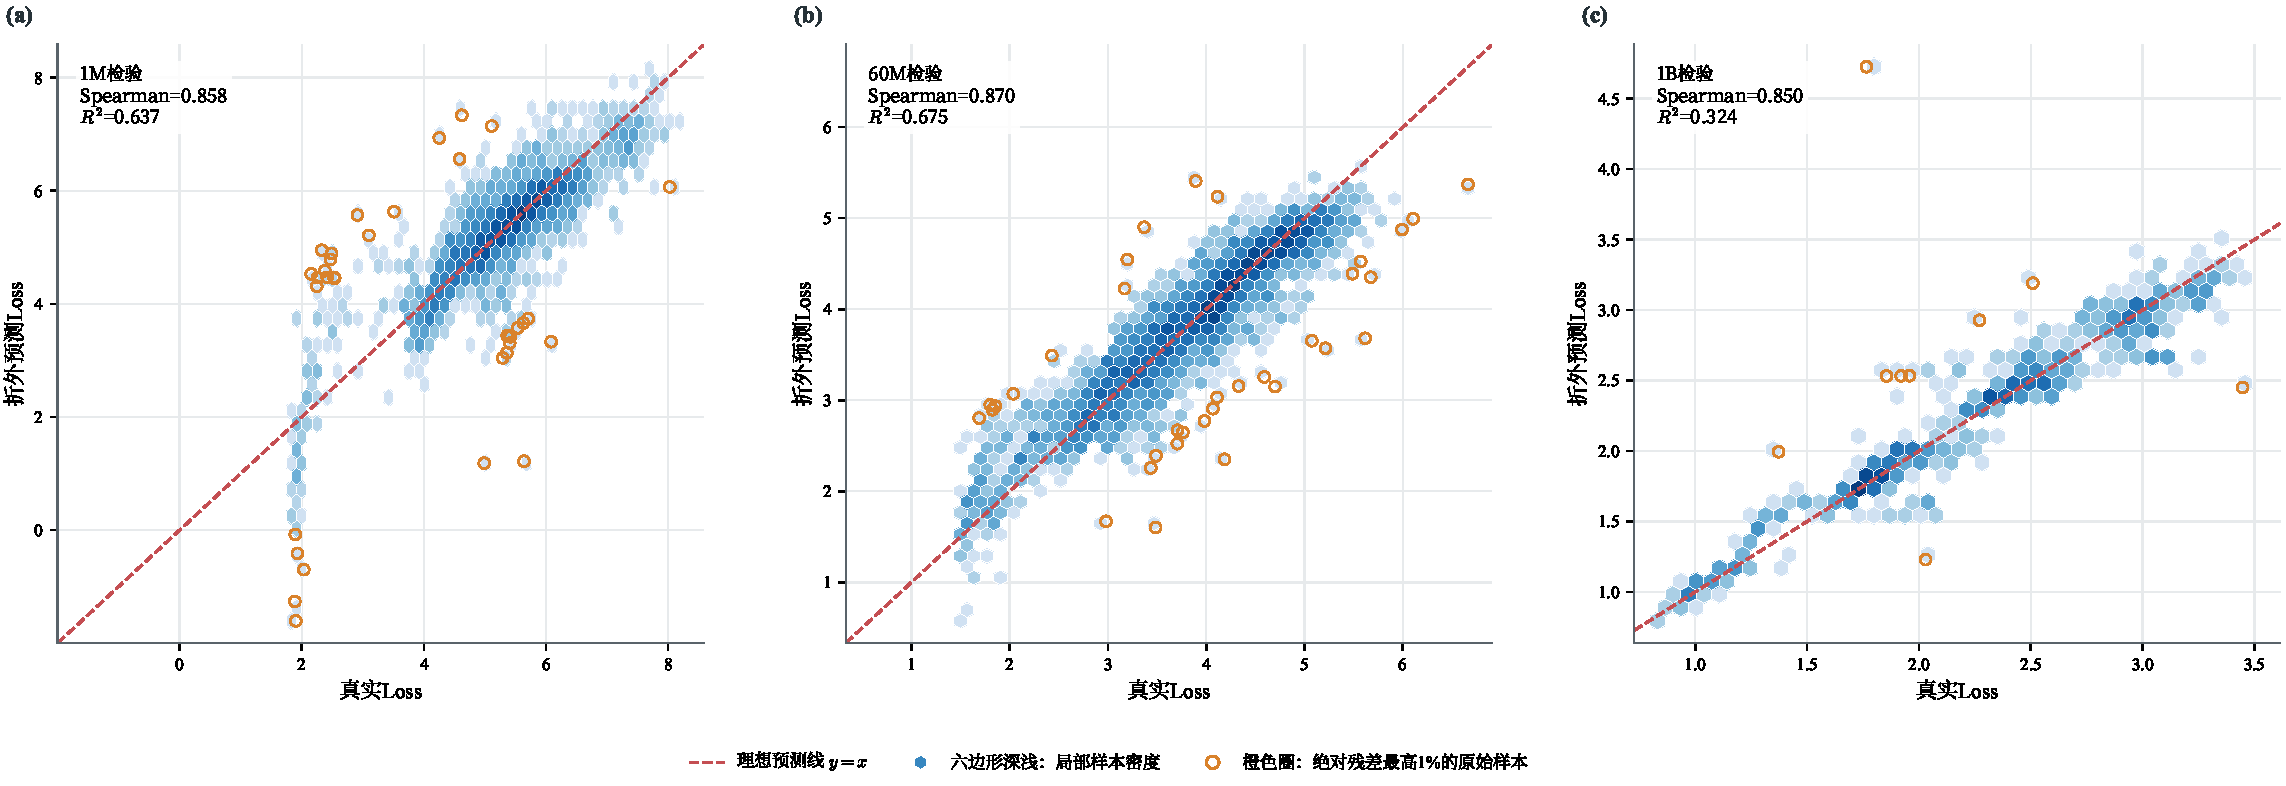
\includegraphics[width=0.98\linewidth]{images/no1/P1_F05_配比模型跨尺度验证.pdf}
\caption{二阶 Scheff\'e--Ridge 模型的跨尺度折外检验}
\label{fig:p1_f05}
\end{figure}

图~\ref{fig:p1_f06}进一步比较领域方向边际收益、两两交互和质量—收益排序。Ubuntu IRC 与 DeepMind Mathematics 的边际收益点估计分别约为 $3.665$ 和 $1.567$，对应 95\% 区间均位于正向 Loss 下降一侧；但其他领域的区间多跨越零，说明局部作用依赖起始配比。136 个领域对的交互中，大量符号在 bootstrap 下并不稳定，故本文只将其作为响应面结构诊断。

领域质量与边际收益的 Spearman、Kendall 系数分别为 $-0.1434$ 和 $-0.1048$，未呈现“质量越高、增配收益越大”的正向单调关系。由于推断域质量本身经过均值回退，且该相关尚无对应区间，结果只能说明静态质量不能代替配比实验，不足以证明二者完全无关。

\begin{figure}[htbp]
\centering
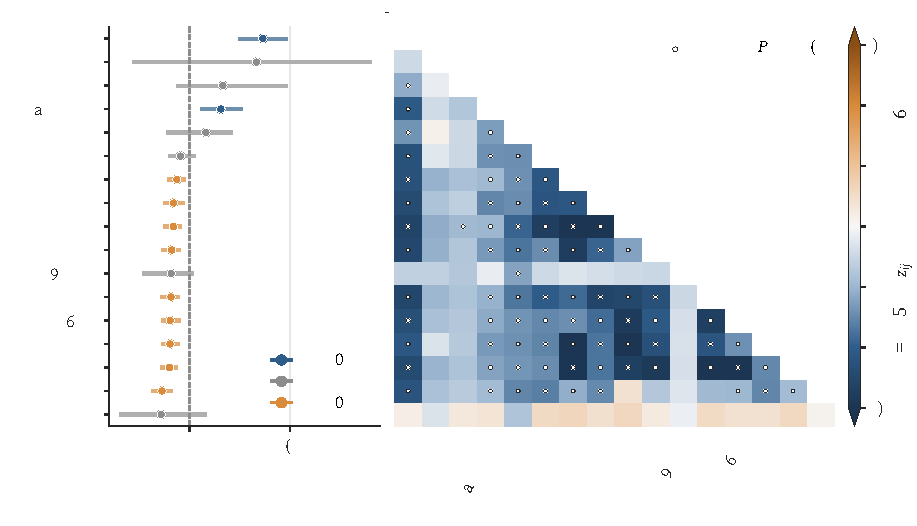
\includegraphics[width=0.98\linewidth]{images/no1/P1_F06_领域边际效应与交互网络.pdf}
\caption{领域边际效应、交互结构与质量—收益排序}
\label{fig:p1_f06}
\end{figure}

\subsubsection{支持域约束下的近优配比}

13 个验证域的 Loss 尺度不同。若直接求平均，高波动领域会主导目标。设训练集中第 $k$ 个验证域 Loss 的四分位距为 $s_k$，定义综合目标
\begin{equation}
J(\boldsymbol p)=\frac{1}{13}\sum_{k=1}^{13}
\frac{\widehat L_k(\boldsymbol p)}{s_k}.
\label{eq:p1_objective}
\end{equation}
四分位距只负责尺度归一化；各验证域在目标中保持等权。

响应面在训练配方附近最可靠。令 $u_i$ 为训练配比第 $i$ 个分量的 $99\%$ 分位，$\boldsymbol\sigma_p$ 为分量标准差，候选配比到训练集的标准化最近距离为 $d(\boldsymbol p)=\min_r\| (\boldsymbol p-\boldsymbol p_r^{\mathrm{train}})/\boldsymbol\sigma_p\|_2$。支持半径 $R$ 取训练点最近邻距离的 $99\%$ 分位，得到可行域
\begin{equation}
\mathcal P=\left\{
\boldsymbol p:
p_i\ge0,\quad \sum_i p_i=1,\quad p_i\le u_i,
\quad d(\boldsymbol p)\le R
\right\}.
\label{eq:p1_support_set}
\end{equation}
最终求解 $\min_{\boldsymbol p\in\mathcal P}J(\boldsymbol p)$。采用 30 个训练配比或其凸组合为起点进行 SLSQP 搜索，并用 10000 个独立随机可行点检查候选目标；在 200 次训练行 bootstrap 中重新拟合响应面并重新优化，用于评估份额不确定性。

表~\ref{tab:p1_optimal}列出点候选中占比最高的八个领域。USPTO backgrounds、PubMed abstracts、Stack Exchange 和 Europarl 合计占 $68.39\%$；但各领域 bootstrap 区间普遍较宽，多数领域存在落到零边界的可能，因此点配比不能脱离区间单独解读。其余九个领域在点候选中的合计占比为 $8.45\%$。

\begin{table}[htbp]
\centering
\small
\setlength{\tabcolsep}{5pt}
\caption{参考近优配比中占比最高的领域}
\label{tab:p1_optimal}
\begin{tabular}{lrrr}
\toprule
领域 & 点候选/\% & bootstrap 95\% 区间/\% & 零边界概率/\% \\
\midrule
USPTO backgrounds & 24.19 & [0.00, 55.61] & 38.0 \\
PubMed abstracts & 18.91 & [0.00, 53.09] & 71.0 \\
Stack Exchange & 14.91 & [0.00, 51.08] & 61.5 \\
Europarl & 10.38 & [0.00, 10.38] & 29.5 \\
Wikipedia (en) & 7.59 & [0.00, 25.85] & 50.5 \\
HackerNews & 7.15 & [0.00, 11.11] & 13.5 \\
PhilPapers & 4.88 & [0.00, 4.88] & 39.0 \\
Pile-CC & 3.55 & [0.00, 27.52] & 74.0 \\
\bottomrule
\end{tabular}
\end{table}

约束回代表明，点候选的比例和为 $1$，最大分量上界违反量仅为 $1.29\times10^{-14}$；支持距离和半径均为 $4.329687$，说明经验支持边界被激活。候选目标为 $4.7651$，优于 10000 个随机可行点中的最佳值 $5.2068$。然而，最佳五个可行起点的目标相对离散度仍为 $1.59\%$，未达到多起点一致性门槛。

图~\ref{fig:p1_f07}从组成空间投影、领域调整幅度和多起点解簇三个角度汇总求解结果。前两条 ILR--PCA 轴仅解释约 $18.05\%$ 的组成变异，二维投影不能代替原始 17 维约束检查；30 个起点中有 28 个得到可行结果，但只有 11 个同时具有正常终止标志。综合支持域边界、起点差异与 bootstrap 区间，本文将 $\boldsymbol p^\star$ 解释为当前响应面和实验范围支持的参考近优配比族，而不宣称其为真实训练空间中的唯一全局最优解。

\begin{figure}[htbp]
\centering
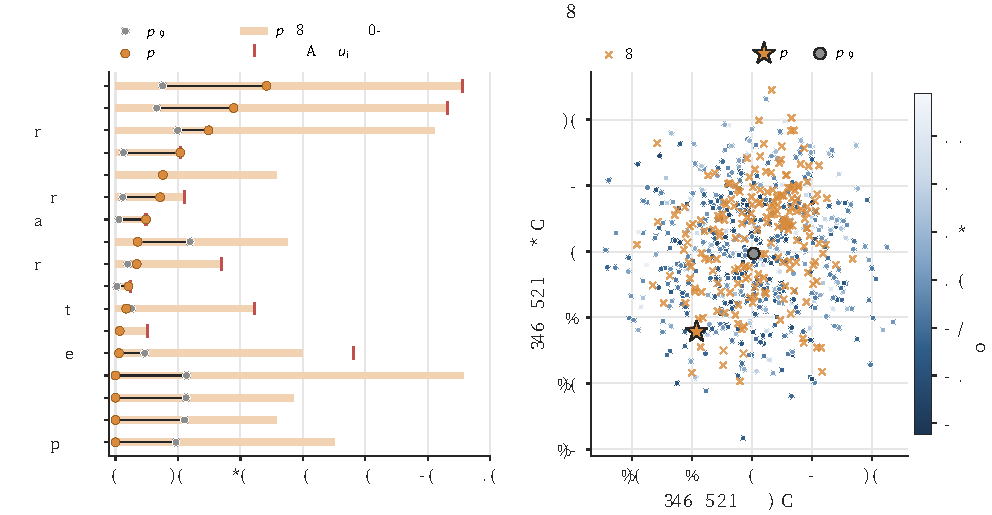
\includegraphics[width=0.98\linewidth]{images/no1/P1_F07_组成空间近优配比与不确定性.pdf}
\caption{组成空间中的参考近优配比及其不确定性}
\label{fig:p1_f07}
\end{figure}

\subsection{敏感性、适用边界与本问输出}

\subsubsection{近优配比的参数敏感性}

为区分“响应面正则强度”与“经验支持域定义”对解的影响，本文分别将支持半径和逐域份额上界的分位数由基准 $99\%$ 调整为 $95\%$、$97.5\%$，并将 Ridge 正则强度调整为 $0.5\alpha^*$ 和 $2\alpha^*$。所有情景均重新执行 30 起点约束优化，而非在基准解附近作线性近似。

图~\ref{fig:p1_f10}(a)显示，收紧支持半径至 $95\%$ 时，基准响应面目标上升 $2.61\%$，配比的 $L_1$ 变化为 $20.12$ 个百分点；将份额上界收紧至 $95\%$ 时，两者分别达到 $3.41\%$ 和 $61.42$ 个百分点。相比之下，$0.5\alpha^*$ 与 $2\alpha^*$ 仅使基准目标增加 $0.006\%$ 和 $0.014\%$，配比变化分别为 $2.77$ 和 $3.93$ 个百分点。图~\ref{fig:p1_f10}(b)进一步表明，约束收紧主要在生物医学全文、生医摘要、专利背景等领域之间重新分配份额，而正则强度扰动下 17 域变化均小于 1 个百分点。

\begin{figure}[htbp]
\centering
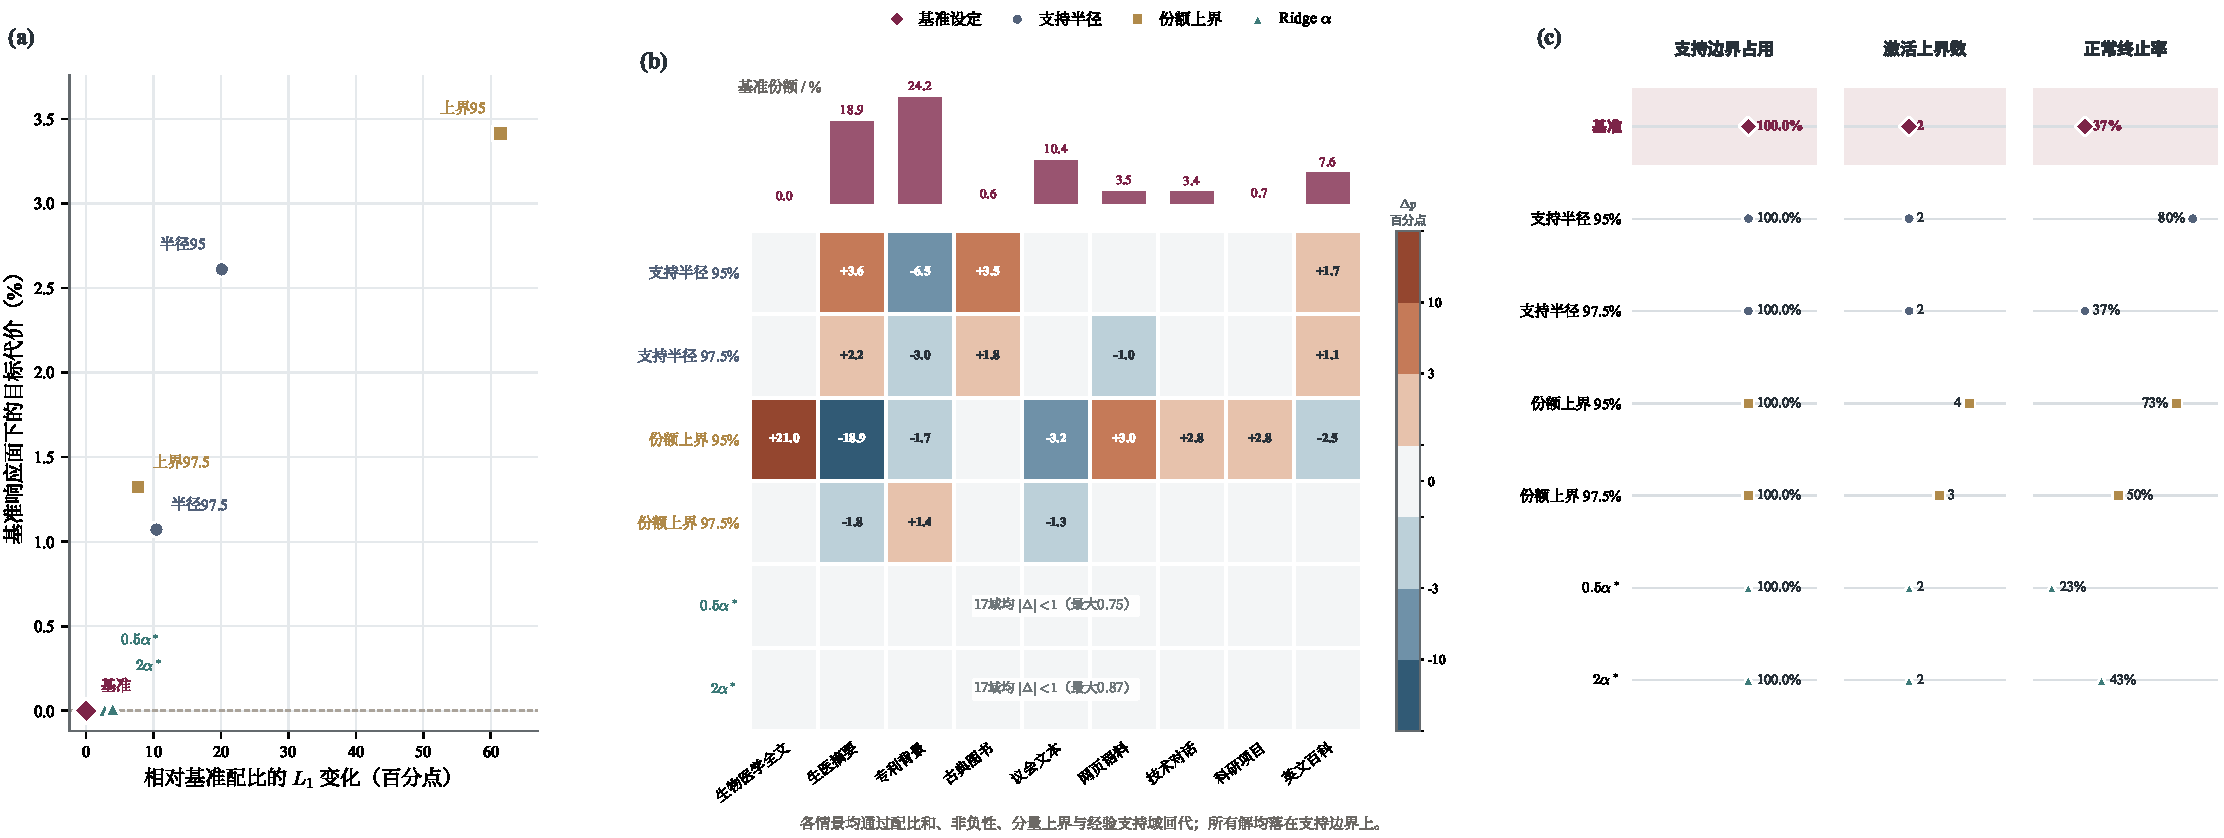
\includegraphics[width=0.99\linewidth]{images/no1/P1_F10_近优配比参数敏感性.pdf}
\caption{近优配比对支持域、份额上界与正则强度的敏感性}
\label{fig:p1_f10}
\end{figure}

七个情景的最优解均落在各自支持边界上，且至少 $28/30$ 个起点可得到可行解；正常终止率则在 $23\%$--$80\%$ 之间。由此可见，正则强度附近的扰动不会实质改变结论，而支持域和份额上界会明显改变点配比。该结果再次支持将 $\boldsymbol p^\star$ 报告为受经验边界约束的近优配比族，而不是唯一且可无条件外推的最优解。

综上，质量模型在统一 22 项异构信号的同时保留了块间冲突，七域质量和扩展集诊断可用于描述领域质量结构；但推断映射不足以支持 11 个领域的细粒度质量排序。二阶 Scheff\'e--Ridge 响应面在 1M、60M 和 1B 实测数据上保持了较好的配比排序能力，局部替换分析进一步说明领域收益依赖参照配方。近优搜索对正则强度较稳健，却明显受支持边界、份额上界和局部解簇影响。

本问向问题二传递的是“可追溯数据属性及其证据边界”，而非无条件的最优配方。具体接口见表~\ref{tab:p1_interface}。其中，$\boldsymbol p_{\mathrm{ref}}$ 是由训练配比样本计算的中性锚点，$\boldsymbol p^\star$ 则是受当前支持域约束的候选近优方案。由于配比改善量在 A、B 两套实验间没有绝对尺度校准，后续主模型优先使用 $\boldsymbol p_{\mathrm{ref}}$，并将 $\boldsymbol p^\star$ 保留为配比迁移的敏感性情景。

\begin{table}[htbp]
\centering
\small
\setlength{\tabcolsep}{5pt}
\caption{问题一向问题二传递的冻结接口}
\label{tab:p1_interface}
\begin{tabular}{p{0.22\linewidth}p{0.36\linewidth}p{0.32\linewidth}}
\toprule
接口 & 含义 & 后续用法 \\
\midrule
$\boldsymbol q$ & $17$ 域质量向量及映射置信边界 & 构造配比加权质量 \\
$\boldsymbol p_{\mathrm{ref}}$ & 训练配比样本的平均组成 & 主标度律的固定配比锚点 \\
$J(\boldsymbol p),R(\boldsymbol p)$ & 标准化综合 Loss 及相对配比响应 & 配比迁移方向与物理门槛检验 \\
$\boldsymbol p^\star$ & 支持域内的参考近优配比族 & 候选方案与敏感性分析 \\
\bottomrule
\end{tabular}
\end{table}
